\chapter{वरण, अपवाह और जातिउद्भव}\label{ch:g12:selection-drift-speciation}

1848 में किसी औद्योगिक शहर के पास काली मिर्च वाले पतंगे का एक काला रूप
पकड़ा गया, जहाँ हर पेड़ का तना कालिख से पुता था; और 1895 तक उस इलाक़े का
लगभग हर पतंगा काला था। एक सदी बाद, कालिख जा चुकी थी और तने फिर फीके थे, तो
वह काला रूप लगभग लुप्त हो चुका था। पतंगों का प्रजनन किसी ने नहीं कराया; वह
छँटाई उन्हें खाते पक्षियों ने की। पिछले दो अध्यायों ने बताया कि विविधता
कैसे उठती है; और यह इस बारे में है कि किसी \omterm{def:g12:selection-drift-speciation:population}{आबादी} में उसका क्या होता है ---
यानी कुछ \omterm{def:g10:universal-dna:gene}{युग्मविकल्पी} वरण से और संयोग से आम कैसे हो जाते हैं और बाक़ी
दुर्लभ --- तथा यह कि आख़िर में एक \omterm{def:g12:selection-drift-speciation:population}{आबादी} दो \omterm{def:g10:biodiversity-scales:species}{जातियाँ} कैसे बनती है।

\section{आबादियाँ और उनके युग्मविकल्पी}

\begin{definition}[आबादी, युग्मविकल्पी बारंबारता]\label{def:g12:selection-drift-speciation:population}
\emph{आबादी}\index{आबादी} किसी एक \omterm{def:g10:biodiversity-scales:species}{जाति} के उन व्यक्तियों का समुच्चय है जो
एक ही जगह रहते हैं और आपस में प्रजनन करते हैं। उसकी आनुवंशिक बनावट हर \omterm{def:g10:universal-dna:gene}{जीन}
के \omterm{def:g10:universal-dna:gene}{युग्मविकल्पियों} की \emph{बारंबारताओं}\index{युग्मविकल्पी
बारंबारता} से वर्णित होती है: दो \omterm{def:g10:universal-dna:gene}{युग्मविकल्पियों} $A$ और $a$ वाले किसी \omterm{def:g10:universal-dna:gene}{जीन}
के लिए, सारी प्रतियों का वह अंश $p$ जो $A$ है और वह अंश $q = 1 - p$ जो $a$
है। इस पैमाने पर विकास एक पीढ़ी से अगली तक \omterm{def:g10:universal-dna:gene}{युग्मविकल्पी} बारंबारताओं का
बदलना है।
\end{definition}

\begin{proposition}[बिना किसी बल के बारंबारताएँ]\label{prop:g12:selection-drift-speciation:hw}
किसी बड़ी \omterm{def:g12:selection-drift-speciation:population}{आबादी} में, जहाँ संगम यादृच्छिक हो, जहाँ कोई \omterm{def:g10:universal-dna:gene}{युग्मविकल्पी} कोई
फ़ायदा न देता हो, और जहाँ न कोई \omterm{def:g11:mutations:mutation}{उत्परिवर्तन} हो न प्रवासन, वहाँ
\omterm{def:g10:universal-dna:gene}{युग्मविकल्पी} बारंबारताएँ पीढ़ी दर पीढ़ी वही रहती हैं, और \omterm{def:g11:enzymes-and-phenotype:phenotype}{जीनप्ररूप} इन
अनुपातों में प्रकट होते हैं
\[
AA : Aa : aa = p^2 : 2pq : q^2 .
\]
यह संदर्भ अवस्था है: पीढ़ियों भर देखा गया इससे कोई भी विचलन इस बात का चिह्न
है कि इनमें से कोई शर्त चूक गई है --- यानी वरण, संयोग, प्रवासन या
\omterm{def:g11:mutations:mutation}{उत्परिवर्तन} काम पर है।
\end{proposition}
\begin{proof}
हर युग्मक $A$ को $p$ प्रायिकता से और $a$ को $q$ प्रायिकता से ढोता है;
यादृच्छिक ढंग से निकाले गए दो युग्मक $AA$ को $p^2$ प्रायिकता से, $aa$ को
$q^2$ से, और $Aa$ को $pq + qp = 2pq$ से देते हैं। नई पीढ़ी के \omterm{def:g10:universal-dna:gene}{युग्मविकल्पी}
गिनने पर: $A$ प्रतियाँ कुल का $p^2 + \tfrac12 (2pq) =
p(p + q) = p$ बनाती हैं। वह बारंबारता अनबदली है।
\end{proof}

\begin{omfigure}
\begin{tikzpicture}[font=\small]
  \draw[thick] (0,0) rectangle (5,5);
  \fill[omDef!25] (0,1.5) rectangle (3.5,5);
  \fill[omProp!25] (3.5,1.5) rectangle (5,5);
  \fill[omProp!25] (0,0) rectangle (3.5,1.5);
  \fill[omThm!30] (3.5,0) rectangle (5,1.5);
  \draw (3.5,0) -- (3.5,5); \draw (0,1.5) -- (5,1.5);
  \node at (1.75,3.25) {$AA$: $p^2$}; \node at (4.25,3.25) {$Aa$: $pq$};
  \node at (1.75,0.75) {$Aa$: $pq$}; \node at (4.25,0.75) {$aa$: $q^2$};
  \node[anchor=south] at (1.75,5.1) {$A$, बारंबारता $p$}; \node[anchor=south] at (4.25,5.1) {$a$, $q$};
  \node[anchor=east] at (-0.1,3.25) {$A$, $p$}; \node[anchor=east] at (-0.1,0.75) {$a$, $q$};
  \node[anchor=south, font=\small\itshape] at (2.5,5.6) {पिता का युग्मक};
  \node[font=\small\itshape, rotate=90, anchor=south] at (-1.1,2.5) {माता का युग्मक};
  \node[anchor=west, align=left, text width=6cm] at (6,2.5) {$p = 0.7$ और $q = 0.3$ के साथ: $AA$ 49\%, $Aa$ 42\%, $aa$ 9\%। किसी आबादी के 9\% में दिखता कोई अप्रभावी लक्षण और 42\% के भीतर चुपचाप ढोया जाता है।};
\end{tikzpicture}

{\small यादृच्छिक संगम के \omterm{def:g11:enzymes-and-phenotype:phenotype}{जीनप्ररूप} अनुपात, क्षेत्रफलों के रूप में। उस वर्ग
की भुजाएँ युग्मक बारंबारताएँ हैं; और चारों आयत \omterm{def:g11:enzymes-and-phenotype:phenotype}{जीनप्ररूप}। विषमयुग्मजी उस
दुर्लभ \omterm{def:g10:universal-dna:gene}{युग्मविकल्पी} की अधिकांश प्रतियाँ थामे हैं।}
\end{omfigure}

\begin{example}[युग्मविकल्पी गिनना]\label{ex:g12:selection-drift-speciation:count}
1000 लोगों में 490 $AA$ हैं, 420 $Aa$ और 90 $aa$। $a$ की प्रतियाँ:
2000 में से $420 + 2 \times 90 = 600$, इसलिए $q = 0.3$ और $p = 0.7$ ---
और \omterm{def:g11:enzymes-and-phenotype:phenotype}{जीनप्ररूप} गिनतियाँ ठीक-ठीक 1000 का $p^2$, $2pq$, $q^2$ हैं: यानी यह
\omterm{def:g12:selection-drift-speciation:population}{आबादी} इस \omterm{def:g10:universal-dna:gene}{जीन} के लिए संदर्भ अवस्था में है। 2500 नवजातों में एक को होती कोई
\omterm{def:g11:genes-and-disease:genetic}{अप्रभावी} बीमारी ($q^2 = 1/2500$) का मतलब $q = 1/50$ और वाहक
$2pq \approx 1/25$: यानी \cref{ch:g11:genes-and-disease} के आँकड़े,
व्युत्पन्न किए हुए।
\end{example}

\section{वरण}

\begin{definition}[प्राकृतिक वरण]\label{def:g12:selection-drift-speciation:selection}
\emph{प्राकृतिक वरण}\index{प्राकृतिक वरण} किसी दिए गए पर्यावरण में
अलग-अलग \omterm{def:g10:universal-dna:gene}{युग्मविकल्पी} ढोते व्यक्तियों के बीच प्रजनन का अंतर है: किसी एक
\omterm{def:g10:universal-dna:gene}{युग्मविकल्पी} के वाहक औसतन किसी दूसरे के वाहकों से अधिक वंशज छोड़ते हैं, और
उस \omterm{def:g10:universal-dna:gene}{युग्मविकल्पी} की बारंबारता पीढ़ी दर पीढ़ी चढ़ती है। जो चुना जाता है वह
पूरा व्यक्ति है --- उसका बचना, उसका संगम, उसकी उर्वरता --- और
\omterm{def:g10:universal-dna:gene}{युग्मविकल्पी} साथ-साथ सवारी करते हैं।
\end{definition}

\begin{proposition}[वरण बारंबारताएँ एक दिशा में बदलता है]\label{prop:g12:selection-drift-speciation:direction}
जिस \omterm{def:g10:universal-dna:gene}{युग्मविकल्पी} के वाहकों की प्रजनन सफलता ज़रा भी अधिक हो वह फैलता है; और
जिसके वाहकों की कम हो वह दुर्लभ हो जाता है। दिशा पर्यावरण तय करता है, और
पर्यावरण पलटे तो वह भी पलट जाती है; रफ़्तार उस फ़ायदे के आकार पर निर्भर है
और इस पर भी कि वह \omterm{def:g10:universal-dna:gene}{युग्मविकल्पी} एक ही प्रति में व्यक्त होता है (\omterm{def:g11:genes-and-disease:genetic}{प्रभावी},
तेज़) या केवल दो में (\omterm{def:g11:genes-and-disease:genetic}{अप्रभावी}, शुरू में धीमा, और कभी पूरी तरह मिटता नहीं,
क्योंकि उसकी दुर्लभ प्रतियाँ विषमयुग्मजियों में छिप जाती हैं)।
\end{proposition}
\begin{proof}[साक्ष्य]
काली मिर्च वाला पतंगा: पक्षी वही पतंगे उठाते हैं जो उन्हें दिखते हैं;
कालिख भरे तनों पर फीका रूप दिखता है, और साफ़ तनों पर गहरा; प्रदूषण के पचास
सालों में गहरे \omterm{def:g10:universal-dna:gene}{युग्मविकल्पी} की बारंबारता लगभग शून्य से चढ़कर 98\% हुई और
साफ़ हवा के चालीस सालों में गिरकर 10\% से नीचे आ गई, ठीक तनों के पीछे।
\omterm{prop:g11:antibiotic-resistance:mechanisms}{प्रतिजैविक प्रतिरोध} (\cref{ch:g11:antibiotic-resistance}): उस दवा की
मौजूदगी में केवल \omterm{prop:g11:antibiotic-resistance:mechanisms}{प्रतिरोधी} \omterm{def:g10:universal-dna:gene}{युग्मविकल्पी} के वाहक ही प्रजनन करते हैं।
लैक्टेज़ की टिकाऊपन (\cref{ch:g11:enzymes-and-phenotype}): वह \omterm{def:g10:universal-dna:gene}{युग्मविकल्पी}
ठीक वहीं आम है जहाँ दूध सहस्राब्दियों से वयस्कों का भोजन रहा है। हर हाल में
\omterm{def:g10:universal-dna:gene}{युग्मविकल्पी} की क़िस्मत पर्यावरण के पीछे चलती है।
\end{proof}

\begin{omfigure}
\begin{tikzpicture}
\begin{axis}[
  width=0.88\linewidth, height=5.6cm,
  axis x line=bottom, axis y line=left,
  xmin=1840, xmax=2000, ymin=0, ymax=110,
  xlabel={वर्ष}, ylabel={गहरे पतंगे (पकड़ का \%)},
  xlabel style={font=\small, at={(axis description cs:0.5,-0.12)}, anchor=north},
  ylabel style={font=\small},
  tick label style={font=\small}, xtick={1850,1875,1900,1925,1950,1975,2000}, ytick={0,25,50,75,100},
  clip=false,
]
\addplot[thick, omThm, mark=*, mark size=1.3pt] coordinates
  {(1848,1) (1860,10) (1870,40) (1880,75) (1895,98) (1920,97) (1950,95) (1960,90) (1970,60) (1980,30) (1990,10) (1998,4)};
\draw[dashed, gray] (axis cs:1956,0) -- (axis cs:1956,105);
\node[font=\scriptsize, anchor=south] at (axis cs:1956,105) {स्वच्छ-वायु क़ानून};
\end{axis}
\end{tikzpicture}

{\small किसी औद्योगिक शहर के पास काली मिर्च वाले पतंगे के गहरे रूप की
बारंबारता (संग्रहालय संग्रहों तथा पकड़ों से गोल की हुई)। वह चढ़ाई तनों के
काले पड़ने के पीछे चलती है; और वह गिरावट उनके साफ़ होने के। पर्यावरण पलटा
तो वरण भी पलट गया।}
\end{omfigure}

\begin{omfigure}
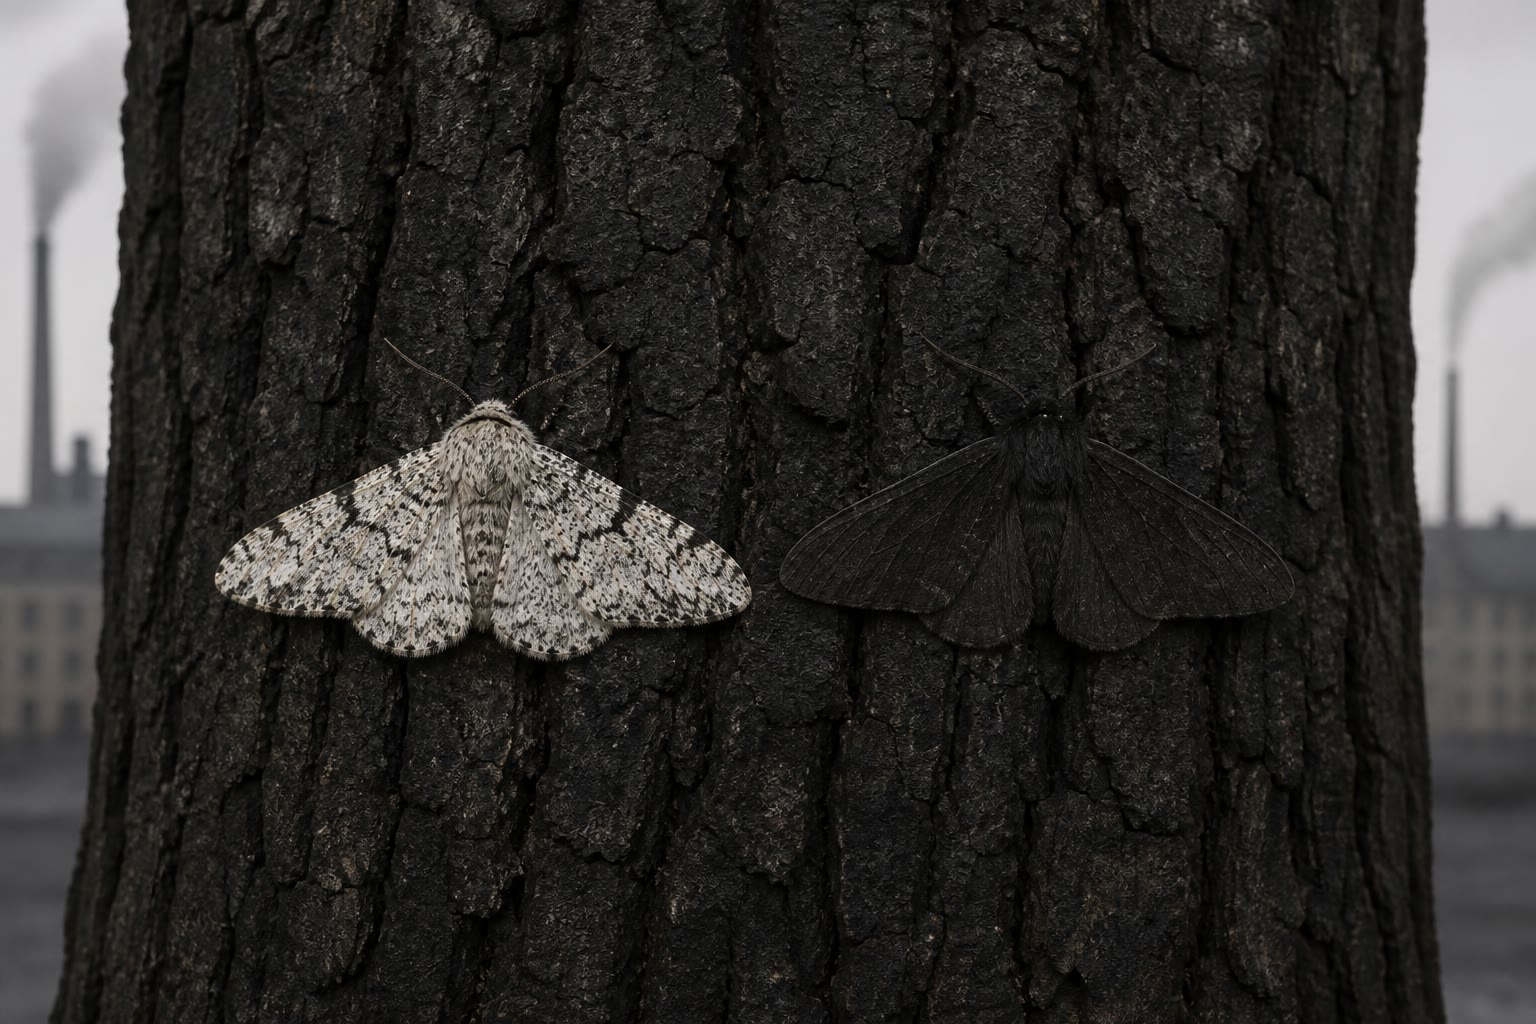
\includegraphics[width=0.6\linewidth]{images/book2/ai/g12-selection-peppered-moths.jpg}

{\small कालिख से काले पड़े किसी तने पर काली मिर्च वाले पतंगे के दोनों रूप।
पक्षी नज़र से शिकार करते हैं: इस छाल पर फीका रूप उठा लिया जाता है और गहरा
बच जाता है; और किसी साफ़, लाइकेन से ढँके तने पर उल्टा।}
\end{omfigure}

\begin{example}[दूसरे लिंग द्वारा वरण]\label{ex:g12:selection-drift-speciation:sexual}
किसी मोर की पूँछ उसे धीमा और शिकारियों को अधिक दिखने वाला बनाती है, फिर भी
वह बची रहती है क्योंकि मोरनियाँ सबसे बड़ी और सबसे नियमित पूँछ वाले नर चुनती
हैं: पूँछ सुधारता कोई \omterm{def:g10:universal-dna:gene}{युग्मविकल्पी} अधिक बार आगे बढ़ता है, चाहे बचने में
उसकी क़ीमत कुछ भी हो। \emph{लैंगिक वरण} --- यानी साथियों का चुनाव ---
जंतुओं के आभूषण, गीत और मुक़ाबले पैदा करता है, और किसी लक्षण को उस दिशा में
धकेल सकता है जिसे अकेला बचाव कभी न पसंद करता।
\end{example}

\section{संयोग: आनुवंशिक अपवाह}

\begin{proposition}[आनुवंशिक अपवाह]\label{prop:g12:selection-drift-speciation:drift}
सीमित आकार की किसी भी \omterm{def:g12:selection-drift-speciation:population}{आबादी} में एक पीढ़ी के \omterm{def:g10:universal-dna:gene}{युग्मविकल्पी} पिछली पीढ़ी का एक
यादृच्छिक प्रतिदर्श होते हैं: कौन-से व्यक्ति संयोग से प्रजनन कर बैठते हैं,
और उनके युग्मक संयोग से कौन-से \omterm{def:g10:universal-dna:gene}{युग्मविकल्पी} ढो बैठते हैं, यह उतार-चढ़ाव
भरा है। इसलिए \omterm{def:g10:universal-dna:gene}{युग्मविकल्पी} बारंबारताएँ बिना किसी फ़ायदे के शामिल हुए पीढ़ी
दर पीढ़ी भटकती हैं --- यानी \emph{आनुवंशिक
अपवाह}\index{आनुवंशिक अपवाह}। \omterm{def:g12:selection-drift-speciation:population}{आबादी} जितनी छोटी, भटकाव उतना बड़ा; किसी छोटी
\omterm{def:g12:selection-drift-speciation:population}{आबादी} में कोई \omterm{def:g10:universal-dna:gene}{युग्मविकल्पी} अकेले संयोग से ही कुछ पीढ़ियों के भीतर खो सकता
है, या 100\% पर पहुँच सकता है, चाहे उसका मोल कुछ भी हो।
\end{proposition}
\begin{proof}[साक्ष्य]
कुछ ही व्यक्तियों की बसाई \omterm{def:g12:selection-drift-speciation:population}{आबादियाँ} --- मुट्ठी भर पक्षियों का बसाया कोई
द्वीप, कुछ दर्जन बाशिंदों से उतरा कोई मानव समुदाय --- स्रोत \omterm{def:g12:selection-drift-speciation:population}{आबादी} के
\omterm{def:g10:universal-dna:gene}{युग्मविकल्पियों} का एक बिगड़ा प्रतिदर्श ढोती हैं: उनमें कोई दुर्लभ बीमारी
\omterm{def:g10:universal-dna:gene}{युग्मविकल्पी} आम हो सकता है, और स्रोत की बहुत-सी विविधता ग़ायब। जो \omterm{def:g10:biodiversity-scales:species}{जातियाँ}
बहुत कम बचे लोगों की किसी \emph{सँकरी गली} से गुज़रीं (\cref{ch:g10:biodiversity-scales}
का चीता, 1890 में बीस जानवरों तक घटा उत्तरी हाथी-सील) वे आज लगभग कोई
\omterm{def:g10:biodiversity-scales:biodiversity}{आनुवंशिक विविधता} नहीं दिखातीं, हज़ारों तक उबर आने के बाद भी। और प्रयोगशाला
में एक ही बारंबारता से शुरू की गईं बहुत-सी छोटी प्रतिकृति \omterm{def:g12:selection-drift-speciation:population}{आबादियाँ} कुछ ही
पीढ़ियों के भीतर हर दिशा में बिखर जाती हैं, जबकि बड़ी \omterm{def:g12:selection-drift-speciation:population}{आबादियाँ} अपनी जगह
टिकी रहती हैं।
\end{proof}

\begin{omfigure}
\begin{tikzpicture}
\begin{axis}[
  width=0.88\linewidth, height=5.8cm,
  axis x line=bottom, axis y line=left,
  xmin=0, xmax=20, ymin=0, ymax=1.05,
  xlabel={पीढ़ी}, ylabel={युग्मविकल्पी $A$ की बारंबारता},
  xlabel style={font=\small, at={(axis description cs:0.5,-0.12)}, anchor=north},
  ylabel style={font=\small},
  tick label style={font=\small}, xtick={0,5,10,15,20}, ytick={0,0.25,0.5,0.75,1},
  legend style={at={(0.5,-0.3)}, anchor=north, legend columns=2, font=\small, draw=none},
]
\addplot[thick, omThm] coordinates {(0,0.5) (1,0.55) (2,0.6) (3,0.5) (4,0.65) (5,0.7) (6,0.6) (7,0.75) (8,0.85) (9,0.8) (10,0.9) (11,0.95) (12,1) (13,1) (14,1) (15,1) (16,1) (17,1) (18,1) (19,1) (20,1)};
\addplot[thick, omThm!60] coordinates {(0,0.5) (1,0.4) (2,0.45) (3,0.3) (4,0.35) (5,0.25) (6,0.3) (7,0.2) (8,0.1) (9,0.15) (10,0.05) (11,0.1) (12,0) (13,0) (14,0) (15,0) (16,0) (17,0) (18,0) (19,0) (20,0)};
\addplot[thick, omThm!35] coordinates {(0,0.5) (1,0.45) (2,0.55) (3,0.6) (4,0.5) (5,0.4) (6,0.45) (7,0.55) (8,0.6) (9,0.7) (10,0.65) (11,0.55) (12,0.5) (13,0.6) (14,0.65) (15,0.75) (16,0.7) (17,0.8) (18,0.75) (19,0.85) (20,0.8)};
\addplot[thick, omDef] coordinates {(0,0.5) (1,0.51) (2,0.49) (3,0.5) (4,0.52) (5,0.51) (6,0.5) (7,0.49) (8,0.48) (9,0.49) (10,0.5) (11,0.51) (12,0.52) (13,0.51) (14,0.5) (15,0.5) (16,0.49) (17,0.5) (18,0.51) (19,0.5) (20,0.5)};
\legend{20 की तीन आबादियाँ, 5000 की एक आबादी}
\end{axis}
\end{tikzpicture}

{\small 50\% से शुरू हुए किसी उदासीन \omterm{def:g10:universal-dna:gene}{युग्मविकल्पी} का नक़ली अपवाह। 20
व्यक्तियों की \omterm{def:g12:selection-drift-speciation:population}{आबादियों} में वह दर्जन भर पीढ़ियों के भीतर स्थिर हो जाता है या
खो जाता है, और हर बार अलग दिशा में; जबकि 5000 की \omterm{def:g12:selection-drift-speciation:population}{आबादी} में वह मुश्किल से
हिलता है।}
\end{omfigure}

\begin{example}[एक संस्थापक प्रभाव]\label{ex:g12:selection-drift-speciation:founder}
किसी द्वीप का समुदाय कुछ दर्जन बाशिंदों ने बसाया था, जिनमें से एक \omterm{def:g11:the-eye:parts}{आँख} की
किसी दुर्लभ गड़बड़ी का \omterm{def:g10:universal-dna:gene}{युग्मविकल्पी} ढोता था। दस पीढ़ियों बाद उस समुदाय में
उस \omterm{def:g10:universal-dna:gene}{युग्मविकल्पी} की बारंबारता दस में एक है --- यानी मुख्य भूमि के मूल्य से
सौ गुना --- क्योंकि तीस संस्थापकों में एक वाहक पहले ही प्रतियों का 1.7\%
है, और किसी छोटी, अलग-थलग \omterm{def:g12:selection-drift-speciation:population}{आबादी} में अपवाह ने उसे और आगे बढ़ा दिया। वह
\omterm{def:g10:universal-dna:gene}{युग्मविकल्पी} कोई फ़ायदा नहीं देता; उसकी बहुतायत इस बात का हादसा है कि नाव
पर कौन चढ़ा।
\end{example}

\begin{method}[वरण या अपवाह?]\label{met:g12:selection-drift-speciation:which}
किसी \omterm{def:g12:selection-drift-speciation:population}{युग्मविकल्पी बारंबारता} के बदलाव के सामने:
\begin{enumerate}
  \item उस \omterm{def:g12:selection-drift-speciation:population}{आबादी} का आकार आँकिए: अपवाह कुछ सौ से नीचे प्रबल है, और लाखों में
        नगण्य।
  \item ऐसी दिशा खोजिए जो पर्यावरण के पीछे चलती हो (वरण), या कोई यादृच्छिक
        चाल (अपवाह)। एक ही ढंग से हिलती प्रतिकृति \omterm{def:g12:selection-drift-speciation:population}{आबादियाँ} वरण बताती हैं;
        और अलग-अलग दिशाओं में हिलतीं, अपवाह।
  \item ऐसी कोई क्रियाविधि खोजिए जो उस \omterm{def:g10:universal-dna:gene}{युग्मविकल्पी} को बचने या प्रजनन से
        जोड़ती हो; ऐसी कोई न हो तो अपवाह पर शक कीजिए।
  \item याद रखिए कि दोनों एक साथ काम करते हैं: वरण एक झुकाव बिठाता है,
        अपवाह शोर जोड़ता है, और छोटी \omterm{def:g12:selection-drift-speciation:population}{आबादियों} में वह शोर उस झुकाव को डुबो
        सकता है।
\end{enumerate}
\end{method}

\section{आबादी से जाति तक}

\begin{proposition}[जातिउद्भव]\label{prop:g12:selection-drift-speciation:speciation}
किसी एक \omterm{def:g10:biodiversity-scales:species}{जाति} की दो \omterm{def:g12:selection-drift-speciation:population}{आबादियाँ} जो \omterm{def:g10:universal-dna:gene}{जीनों} का लेन-देन बंद कर दें --- भूगोल,
बरताव या समय की किसी रुकावट से अलग होकर --- वे अलग-अलग विकसित होती हैं: हर
एक अपने \omterm{def:g11:mutations:mutation}{उत्परिवर्तन} जमा करती है, अपने पर्यावरण से चुनी जाती है और अपने ढंग
से अपवाहित होती है। जब वह अपसरण इतना आगे बढ़ चुका हो कि दोनों \omterm{def:g12:selection-drift-speciation:population}{आबादियों} के
व्यक्ति फिर मिलने पर भी आपस में प्रजनन न करें, या बंध्य संतान दें, तब जहाँ
एक \omterm{def:g10:biodiversity-scales:species}{जाति} थी वहाँ दो होती हैं। \emph{जातिउद्भव}\index{जातिउद्भव} यही
प्रक्रिया है; इसमें आम तौर पर हज़ारों से लेकर लाखों पीढ़ियाँ लगती हैं,
हालाँकि \omterm{prop:g12:diversification-of-life:polyploidy}{बहुगुणिता} (\cref{ch:g12:diversification-of-life}) इसे एक ही में पा
लेती है।
\end{proposition}
\begin{proof}[साक्ष्य]
द्वीप: गैलापागोस के हर द्वीप पर उसके अपने फिंच हैं, जो किसी मुख्य भूमि \omterm{def:g10:biodiversity-scales:species}{जाति}
से उतरे हैं और पड़ोसी द्वीपों वालों के सबसे पास हैं। झीलें: किसी एक पूर्वज
सिक्लिड मछली ने अफ़्रीका की एक झील में कुछ ही लाख सालों के भीतर सैकड़ों
\omterm{def:g10:biodiversity-scales:species}{जातियाँ} दी हैं, जो आवास से और नर के रंग को लेकर मादाओं के चुनाव से अलग हुईं।
वलय \omterm{def:g10:biodiversity-scales:species}{जातियाँ}: किसी गल की \omterm{def:g12:selection-drift-speciation:population}{आबादियाँ} आर्कटिक के चारों ओर फैलीं, और पूरे गोल में
अपने पड़ोसियों से प्रजनन करती रहीं, जब तक दोनों सिरे यूरोप में ऐसे रूपों की
तरह न मिले जो आपस में प्रजनन नहीं करते --- यानी \omterm{def:g10:biodiversity-scales:species}{जाति} की एक सीमा, बनते वक़्त
पकड़ी गई। और हाल ही में अलग हुई \omterm{def:g10:biodiversity-scales:species}{जातियाँ}, जैसे ध्रुवीय और भूरे भालू, आज भी
कभी-कभी उर्वर संकर देती हैं: वह सीमा मात्रा का मामला है।
\end{proof}

\begin{omfigure}
\begin{tikzpicture}[font=\small, >=Stealth]
  % one population
  \draw[thick, fill=omDef!12] (0,0) ellipse (1.4 and 0.8);
  \node at (0,0) {एक आबादी};
  \draw[->, thick] (1.6,0) -- (2.6,0) node[midway, above, font=\scriptsize, align=center] {रुकावट\\ आती है};
  % two separated
  \draw[thick, fill=omDef!12] (4.0,0.9) ellipse (1.2 and 0.6); \node at (4.0,0.9) {आबादी 1};
  \draw[thick, fill=omDef!12] (4.0,-0.9) ellipse (1.2 and 0.6); \node at (4.0,-0.9) {आबादी 2};
  \draw[very thick, gray] (2.7,0) -- (5.3,0);
  \draw[->, thick] (5.5,0) -- (6.5,0) node[midway, above, font=\scriptsize, align=center] {अलग-अलग\\ विकास};
  % diverged
  \draw[thick, fill=omMeth!15] (7.9,0.9) ellipse (1.2 and 0.6); \node at (7.9,0.9) {उत्परिवर्तन 1};
  \draw[thick, fill=omThm!15] (7.9,-0.9) ellipse (1.2 and 0.6); \node at (7.9,-0.9) {उत्परिवर्तन 2};
  \node[font=\scriptsize, align=center] at (7.9,0.0) {अपना वरण,\\ अपना अपवाह};
  \draw[->, thick] (9.3,0) -- (10.3,0) node[midway, above, font=\scriptsize, align=center] {रुकावट\\ हटी};
  % two species
  \draw[thick, fill=omMeth!15] (11.6,0.7) ellipse (1.1 and 0.55); \node at (11.6,0.7) {जाति 1};
  \draw[thick, fill=omThm!15] (11.6,-0.7) ellipse (1.1 and 0.55); \node at (11.6,-0.7) {जाति 2};
  \node[font=\scriptsize, align=center] at (11.6,0.0) {कोई अंतःप्रजनन नहीं};
\end{tikzpicture}

{\small अलगाव से \omterm{prop:g12:selection-drift-speciation:speciation}{जातिउद्भव}। कोई रुकावट किसी \omterm{def:g12:selection-drift-speciation:population}{आबादी} को चीर देती है; हर आधा
अपने बल पर विकसित होता है; और जब वे फिर मिलते हैं तो आपस में प्रजनन नहीं
करते। वह रुकावट कोई जलडमरूमध्य, कोई पहाड़, आवास का कोई बदलाव, या संगम की
कोई पसंद हो सकती है।}
\end{omfigure}

\begin{proposition}[जाति, दोबारा सोची गई]\label{prop:g12:selection-drift-speciation:concept}
\omterm{def:g10:biodiversity-scales:species}{जाति} एक \omterm{def:g12:selection-drift-speciation:population}{आबादी} है, या \omterm{def:g12:selection-drift-speciation:population}{आबादियों} का एक समुच्चय, जिसके सदस्य आपस में प्रजनन
करते हैं और ऐसे बाक़ी समुच्चयों से आनुवंशिक रूप से अलग-थलग हैं --- यानी ऐसी
परिभाषा जो किसी दिए गए क्षण पर अधिकांश जंतुओं और पौधों के लिए चलती है, पर
जिसके किनारे हैं: अलग होने की प्रक्रिया में पड़ी \omterm{def:g12:selection-drift-speciation:population}{आबादियाँ}, वे \omterm{def:g10:biodiversity-scales:species}{जातियाँ} जो अब
भी संकरित होती हैं, वे जीव जो बिना लैंगिकता के जनन करते हैं। कोई \omterm{def:g10:biodiversity-scales:species}{जाति} कोई
जमा हुआ प्रकार नहीं बल्कि समय में एक वंशरेखा है: वह तब शुरू होती है जब कोई
\omterm{def:g12:selection-drift-speciation:population}{आबादी} अलग-थलग हो जाए, तब तक रहती है जब तक उसके सदस्य आपस में प्रजनन करते
रहें, और विलुप्ति से या नई \omterm{def:g10:biodiversity-scales:species}{जातियों} में चिरने से ख़त्म होती है। आज जीवित
\omterm{def:g10:biodiversity-scales:species}{जातियाँ} उस वृक्ष के सिरे हैं जिसकी शाखाएँ
\cref{ch:g12:phylogenetic-trees} का विषय हैं।
\end{proposition}
\admitted

\begin{remark}[विकास, जोड़कर देखा गया]\label{rem:g12:selection-drift-speciation:assembled}
\omterm{def:g11:mutations:mutation}{उत्परिवर्तन} और फेंटाई विविधता जुटाते हैं; द्विगुणन, अंतरण, \omterm{prop:g12:diversification-of-life:polyploidy}{बहुगुणिता}, नियमन
और \omterm{def:g12:diversification-of-life:symbiosis}{सहजीविता} और जुटाते हैं; वरण उसे पर्यावरण के हिसाब से छाँटता है, और अपवाह
संयोग से; अलगाव \omterm{def:g12:selection-drift-speciation:population}{आबादियों} को तब तक अपसरित होने देता है जब तक वे \omterm{def:g10:biodiversity-scales:species}{जातियाँ} न बन
जाएँ; और विलुप्ति उन्हें हटा देती है। इनमें से किसी क़दम का कोई लक्ष्य नहीं
है, और कोई आगे नहीं देखता; फिर भी मिलकर, जीवाश्म अभिलेख के चार अरब सालों
पर, उन्होंने \cref{ch:g10:biodiversity-scales} की विविधता बनाई है। जो
सिद्धांत इन क़दमों और उनके आपसी खेल का नाम लेता है वही विकास का सिद्धांत
है, और इस साल का हर अध्याय उसके साक्ष्य का एक टुकड़ा रहा है।
\end{remark}

\section{अभ्यास}

\begin{exercise}[$\star$]\label{exo:g12:selection-drift-speciation:1}
\omterm{def:g12:selection-drift-speciation:population}{युग्मविकल्पी बारंबारता} की परिभाषा दीजिए, और $p = 0.8$ के साथ संदर्भ अवस्था
में बैठी किसी \omterm{def:g12:selection-drift-speciation:population}{आबादी} के \omterm{def:g11:enzymes-and-phenotype:phenotype}{जीनप्ररूप} अनुपात बताइए।
\end{exercise}

\begin{exercise}[$\star$]\label{exo:g12:selection-drift-speciation:2}
\omterm{def:g12:selection-drift-speciation:selection}{प्राकृतिक वरण} और \omterm{prop:g12:selection-drift-speciation:drift}{आनुवंशिक अपवाह} की परिभाषा दीजिए, और उनके बीच का असल अंतर
बताइए।
\end{exercise}

\begin{exercise}[$\star$]\label{exo:g12:selection-drift-speciation:3}
पतंगे वाले चित्र से 1880 में और 1980 में गहरे रूप की बारंबारता पढ़िए, और हर
एक के पीछे के पर्यावरणीय बदलाव का नाम लीजिए।
\end{exercise}

\begin{exercise}[$\star$]\label{exo:g12:selection-drift-speciation:4}
किसी छोटी \omterm{def:g12:selection-drift-speciation:population}{आबादी} में अपवाह अधिक क्यों मायने रखता है?
\end{exercise}

\begin{exercise}[$\star$]\label{exo:g12:selection-drift-speciation:5}
एक \omterm{def:g12:selection-drift-speciation:population}{आबादी} को दो \omterm{def:g10:biodiversity-scales:species}{जातियाँ} बनने के लिए क्या चाहिए?
\end{exercise}

\begin{exercise}[$\star\star$]\label{exo:g12:selection-drift-speciation:6}
500 की किसी \omterm{def:g12:selection-drift-speciation:population}{आबादी} में 320 $AA$ हैं, 160 $Aa$ और 20 $aa$। $p$ और $q$
निकालिए, फिर संदर्भ अवस्था पर अपेक्षित \omterm{def:g11:enzymes-and-phenotype:phenotype}{जीनप्ररूप} संख्याएँ, और तुलना कीजिए।
\end{exercise}

\begin{exercise}[$\star\star$]\label{exo:g12:selection-drift-speciation:7}
किसी \omterm{def:g11:genes-and-disease:genetic}{अप्रभावी} \omterm{def:g10:universal-dna:gene}{युग्मविकल्पी} की बारंबारता 0.01 है। \omterm{def:g12:selection-drift-speciation:population}{आबादी} का कौन-सा अंश वह
\omterm{def:g11:genes-and-disease:genetic}{अप्रभावी} लक्षण दिखाता है, और कौन-सा अंश उस \omterm{def:g10:universal-dna:gene}{युग्मविकल्पी} को बिना दिखे ढोता
है? उस लक्षण के ख़िलाफ़ वरण से वह \omterm{def:g10:universal-dna:gene}{युग्मविकल्पी} मिटाना इतना मुश्किल क्यों है?
\end{exercise}

\begin{exercise}[$\star\star$]\label{exo:g12:selection-drift-speciation:8}
अपवाह वाले चित्र से बताइए कि सिरों तक पहुँची दोनों छोटी \omterm{def:g12:selection-drift-speciation:population}{आबादियों} में वह
\omterm{def:g10:universal-dna:gene}{युग्मविकल्पी} कितनी पीढ़ियों में स्थिर हुआ या खो गया? तीसरी में क्यों नहीं?
\end{exercise}

\begin{exercise}[$\star\star$]\label{exo:g12:selection-drift-speciation:9}
समझाइए कि कालिख वाले दशकों में काली मिर्च वाले पतंगे का गहरा \omterm{def:g10:universal-dna:gene}{युग्मविकल्पी}
100\% तक क्यों नहीं पहुँचा, और इसके लिए उन पतंगों का इस्तेमाल कीजिए जो
देहात में रहते और प्रजनन करते हैं।
\end{exercise}

\begin{exercise}[$\star\star$]\label{exo:g12:selection-drift-speciation:10}
बीस सील किसी सँकरी गली से बच निकले; अब उस \omterm{def:g10:biodiversity-scales:species}{जाति} की संख्या 100\,000 है पर वह
लगभग कोई \omterm{def:g10:biodiversity-scales:biodiversity}{आनुवंशिक विविधता} नहीं दिखाती। अपवाह से समझाइए।
\end{exercise}

\begin{exercise}[$\star\star$]\label{exo:g12:selection-drift-speciation:11}
\cref{met:g12:selection-drift-speciation:which} को दो मामलों पर लगाइए: किसी
नए शिकारी के आने के बाद झील की दस अलग-अलग \omterm{def:g12:selection-drift-speciation:population}{आबादियों} में एक साथ चढ़ता कोई
\omterm{def:g10:universal-dna:gene}{युग्मविकल्पी}; और तीस पक्षियों की किसी एक द्वीप \omterm{def:g12:selection-drift-speciation:population}{आबादी} में 80\% पर पहुँचता
कोई \omterm{def:g10:universal-dna:gene}{युग्मविकल्पी}।
\end{exercise}

\begin{exercise}[$\star\star\star$]\label{exo:g12:selection-drift-speciation:12}
मलेरिया वाले किसी इलाक़े में हँसियाकार \omterm{def:g10:universal-dna:gene}{युग्मविकल्पी} की बारंबारता 0.15 है
हालाँकि $aa$ बच्चे शायद ही बचते हैं। \omterm{def:g11:enzymes-and-phenotype:phenotype}{जीनप्ररूप} अनुपातों की मदद से $AA$,
$Aa$ और $aa$ नवजातों के अंश निकालिए, और समझाइए कि मलेरिया के ख़िलाफ़ $Aa$
का फ़ायदा $aa$ के नुक़सान के बावजूद उस \omterm{def:g10:universal-dna:gene}{युग्मविकल्पी} को आम कैसे बनाए रखता
है।
\end{exercise}

\begin{exercise}[$\star\star\star$]\label{exo:g12:selection-drift-speciation:13}
किसी एक झील की दो सिक्लिड \omterm{def:g10:biodiversity-scales:species}{जातियाँ} मुख्यतः नरों के रंग में अलग हैं, और हर
एक की मादाएँ अपना ही रंग चुनती हैं। गँदले पानी में, जहाँ रंग नहीं दिखते, वे
दोनों आज़ादी से संकरित होती हैं। उन \omterm{def:g10:biodiversity-scales:species}{जातियों} को क्या अलग-थलग रखता है, और
गँदले वाला मामला यह अलगाव कितना हाल का है इस बारे में क्या कहता है?
\end{exercise}

\begin{exercise}[$\star\star\star$]\label{exo:g12:selection-drift-speciation:14}
समझाइए कि गलों की वलय \omterm{def:g10:biodiversity-scales:species}{जाति} यह तर्क क्यों है कि \omterm{prop:g12:selection-drift-speciation:speciation}{जातिउद्भव} क्रमिक होता है,
और यूरोप में मिलते दोनों सिरे फिर भी दो \omterm{def:g10:biodiversity-scales:species}{जातियाँ} क्यों कहलाते हैं।
\end{exercise}

\begin{exercise}[$\star\star\star$]\label{exo:g12:selection-drift-speciation:15}
``वरण जीवों को बेहतर बनाता है।'' एक अनुच्छेद में विवेचना कीजिए: किस बात में
बेहतर, कहाँ, और किसके मुक़ाबले; और अपवाह, पलटाव तथा लैंगिक वरण उसमें क्या
जोड़ते हैं।
\end{exercise}

\section{समस्या: उस द्वीप के चूहे}

\begin{problem}[{सप्ताहांत समस्या --- किसी द्वीप पर चूहों की एक आबादी:
उसकी युग्मविकल्पी बारंबारताएँ निकाली गईं, किसी नए शिकारी का वरण पीछा किया
गया, किसी नन्ही बस्ती का अपवाह नक़ली रूप से चलाया गया, और एक जाति का जन्म
पहले से देखा गया}]
\label{pb:g12:selection-drift-speciation:1}
किसी चट्टानी द्वीप पर चूहे कोट के रंग का एक \omterm{def:g10:universal-dna:gene}{जीन} ढोते हैं जिसके दो
\omterm{def:g10:universal-dna:gene}{युग्मविकल्पी} हैं: $D$ (गहरा, \omterm{def:g11:genes-and-disease:genetic}{प्रभावी}) और $d$ (फीका)। 2000 चूहों की एक
गणना में \omterm{def:g11:enzymes-and-phenotype:phenotype}{जीनप्ररूप} $DD$ वाले 720 गहरे चूहे, 960 गहरे $Dd$, और 320 फीके
$dd$ मिलते हैं।

\medskip
\noindent\textbf{भाग I --- अभी की \omterm{def:g12:selection-drift-speciation:population}{आबादी}।}
\begin{enumerate}
  \item प्रतियाँ गिनकर $p$ यानी $D$ की और $q$ यानी $d$ की बारंबारताएँ
        निकालिए।
  \item संदर्भ अवस्था पर अपेक्षित \omterm{def:g11:enzymes-and-phenotype:phenotype}{जीनप्ररूप} संख्याएँ निकालिए और उस गणना से
        तुलना कीजिए। क्या वह \omterm{def:g12:selection-drift-speciation:population}{आबादी} संदर्भ अवस्था में है?
  \item गहरे चूहों का कौन-सा अंश $d$ का वाहक है?
  \item पिछले जवाब से समझाइए कि एक पीढ़ी के लिए सारे फीके चूहे द्वीप से हटा
        देना $q$ को ज़रा ही क्यों घटाएगा। ऐसे किसी हटाव के बाद का नया $q$
        निकालिए, यदि बचे चूहे यादृच्छिक ढंग से प्रजनन करें।
  \item संदर्भ अवस्था की चारों शर्तों में से कौन-सी किसी छोटे द्वीप पर
        चूकने की सबसे अधिक संभावना रखती है, और किस असर के साथ?
\end{enumerate}

\medskip
\noindent\textbf{भाग II --- एक शिकारी आता है।}
उल्लू उस द्वीप पर बस जाते हैं। फीकी चट्टान पर गहरे चूहे दोगुनी बार दिखते
और खाए जाते हैं: हर पीढ़ी में आधे गहरे चूहे प्रजनन से पहले मर जाते हैं जबकि
सारे फीके चूहे बच जाते हैं।
\begin{enumerate}[resume]
  \item गणना की संख्याओं से शुरू करके निकालिए कि पहली पीढ़ी में हर
        \omterm{def:g11:enzymes-and-phenotype:phenotype}{जीनप्ररूप} के कितने चूहे प्रजनन तक बचते हैं।
  \item बचे चूहों में $p$ और $q$ निकालिए।
  \item बचे चूहे यादृच्छिक ढंग से संगम करें तो अगली पीढ़ी के \omterm{def:g11:enzymes-and-phenotype:phenotype}{जीनप्ररूप}
        अनुपात निकालिए, फिर उल्लू दोबारा लगाइए और उसके बचे चूहों में $q$
        निकालिए।
  \item एक बार और दोहराइए (दो सार्थक अंक)। तीनों पीढ़ियों पर $q$ का झुकाव
        बताइए।
  \item समझाइए कि $q$ लगातार क्यों चढ़ता है, और उसी वरण के नीचे किसी
        \omterm{def:g11:genes-and-disease:genetic}{अप्रभावी} \omterm{def:g10:universal-dna:gene}{युग्मविकल्पी} के उलट $D$ पूरी तरह क्यों मिटाया जा सकता है।
\end{enumerate}

\medskip
\noindent\textbf{भाग III --- छह की एक बस्ती।}
कोई तूफ़ान छह चूहे किसी पड़ोसी टापू तक ले जाता है: 2 $DD$, 3 $Dd$, 1 $dd$।
\begin{enumerate}[resume]
  \item उस बस्ती में $q$ निकालिए और द्वीप से तुलना कीजिए।
  \item पहली बार में, संयोग से, केवल वे दो $DD$ और एक $Dd$ प्रजनन करते
        हैं। अगली पीढ़ी में $q$ के संभव मान क्या हैं? उस \omterm{def:g12:selection-drift-speciation:population}{आबादी} की विविधता
        का क्या हुआ?
  \item समझाइए कि उस टापू पर कोई \omterm{def:g10:universal-dna:gene}{युग्मविकल्पी} बिना उल्लुओं या किसी फ़ायदे
        के कुछ ही पीढ़ियों में क्यों ग़ायब हो सकता है।
  \item उस टापू पर कोई उल्लू नहीं है। वहाँ $d$ की क़िस्मत का अनुमान
        लगाइए, और बताइए कि दो पड़ोसी द्वीप बिना अनुकूलन के किसी कारण के
        अलग-अलग कोट रंगों पर क्यों ख़त्म हो सकते हैं।
  \item उस प्रक्रिया का नाम दीजिए, और उस बस्ती का वह लक्षण भी जो उसे वहाँ
        हावी बनाता है।
\end{enumerate}

\medskip
\noindent\textbf{भाग IV --- दस हज़ार साल बाद।}
उस टापू के चूहे, अलग-थलग रहकर, अपसरित हो चुके हैं: छोटे, अधिक फीके, और किसी
और मौसम में प्रजनन करते। प्रयोगशाला में द्वीप के चूहों के साथ रखे जाने पर
वे शायद ही संगम करते हैं, और जो थोड़े संकर बनते हैं वे बंध्य होते हैं।
\begin{enumerate}[resume]
  \item क्या उस टापू के चूहे एक नई \omterm{def:g10:biodiversity-scales:species}{जाति} हैं? उस परिभाषा से उचित ठहराइए।
  \item उस रुकावट का नाम लीजिए जिसने यह प्रक्रिया शुरू की और उन दो
        क्रियाविधियों का भी जिन्होंने वह अपसरण चलाया।
  \item दोनों के बीच प्रजनन का मौसम अलग है। समझाइए कि ऐसा अंतर, एक बार
        मौजूद हो जाए, तो वह अलगाव को कैसे पुख़्ता करता है।
  \item यदि वह टापू कल फिर उस द्वीप से जुड़ जाए, तो क्या वे दोनों वापस एक
        \omterm{def:g12:selection-drift-speciation:population}{आबादी} में मिल जाएँगे? सवाल 17 के मामले को किसी पहले चरण से, मान
        लीजिए 100 साल बाद वाले से, अलग कीजिए।
  \item परिणाम लिखिए: उल्लुओं की तीन पीढ़ियों से पहले और बाद उस द्वीप पर
        $d$ की बारंबारता, उस टापू पर $d$ की क़िस्मत और उसके लिए ज़िम्मेदार
        प्रक्रिया, तथा आख़िर में \omterm{def:g10:biodiversity-scales:species}{जातियों} की संख्या।
\end{enumerate}
\end{problem}
